\documentclass{article}
\usepackage[utf8]{inputenc}
\usepackage{tikz}
\usetikzlibrary{shapes,arrows}
\usepackage[ruled,vlined]{algorithm2e}
%\usepackage{algpseudocode}
\usepackage{multicol}
\renewcommand{\contentsname}{{\Huge Table de Matières}}
\usepackage{titlesec}
\usepackage{xcolor}
\usepackage{listings}
\usepackage{graphicx}
\titleformat{\section}{\huge\bfseries}{\thesection}{1em}{}
\titleformat{\subsection}{\LARGE\bfseries}{\thesubsection}{1em}{}
\titleformat{\subsubsection}{\Large\bfseries}{\thesubsubsection}{1em}{}
\begin{document}
%first page
\begin{center}
\pagenumbering{gobble}
\linespread{2.0}\selectfont

{\Huge U}{\huge NIVERSITÉ DE }{\Huge M}{\huge ONTPELLIER}\\
{\huge L2}{\LARGE ~INFORMATIQUE }
\\~\\~\\~\\~\\
{\Large\textbf{GOLF MATHÉMATIQUE}}
\\~\\~\\~\\~\\

\linespread{1}\selectfont

RAPPORT DE PROJET T.E.R\\
PROJET INFORMATIQUE HLIN405\\
\vfill
\end{center}
\begin{multicols}{2}
\begin{flushleft}
\textbf{Etudiants:}\\
~~M. Mike Germain\\
~~M. Benjamin Baska\\
~~M. Kevin Lastra
\end{flushleft}
\columnbreak
\begin{flushright}
\textbf{Encadrante:}\\
~~Mme. Annie Chateau
\end{flushright}
\end{multicols}
\newpage
%bilan
\pagenumbering{arabic}
\setcounter{page}{1}
\tableofcontents
\newpage
%introduction
{\textbf{\Huge Introduction}}\\~\\~\\
~~Sous la direction de Mme. Annie Chateau, notre groupe, composé de Mike Germain, Benjamin Baska, Kevin Lastra, a travaillé sur le développement du jeu "Golf Mathématique" comme projet du module HLIN405.

\newpage
%cahier de charges
\section{Organisation du projet}
\subsection{Objectifs et cahier des charges}
~\\~\\
Le but est de créer un jeu de golf, version mathématique.
\\~\\
\textbf{\large Base et Règles}
\\~\\
Les règles sont simple:
\\~\\
- Partir du point de départ et aller jusqu'au trou en faisant le moins de coup.
\\~\\
- Pour se déplacer, on ne peut que de la portée indiqué sur notre case, dans 8 positions différentes, haut, bas, droite, gauche, ainsi que, haut droite, haut gauche, bas droite, bas gauche.
\\~\\
\textbf{\large Interface Graphique}
\\~\\
Pour la partie graphique, le but est d'apprendre à utiliser une interface graphique.
\\~\\
\textbf{\large Génération automatique de la carte}
\\~\\
x2
\\~\\
\textbf{\large Intelligence Artificielle}
\\~\\
au secours
\\~\\
\newpage
\subsection{Division du travail}
~\\~\\~\\~\\~\\~\\~\\~\\
\tikzstyle{decision} = [diamond, draw, fill=blue!20, 
    text width=4.5em, text badly centered, node distance=3cm, inner sep=0pt]
\tikzstyle{block} = [rectangle, draw, fill=blue!20, 
    text width=5em, text centered, rounded corners, minimum height=4em]
\tikzstyle{line} = [draw, -latex']
\tikzstyle{cloud} = [draw, ellipse,fill=red!20, node distance=3cm,
    minimum height=2em]

\begin{figure}[h]
\centering
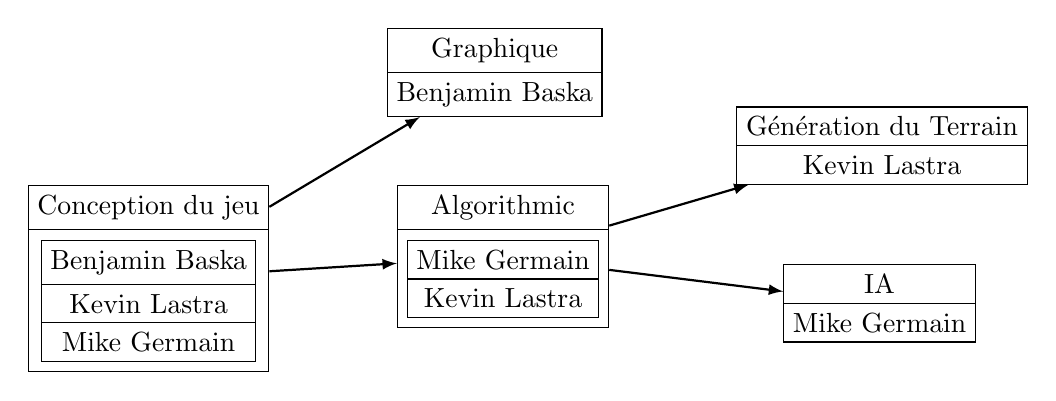
\begin{tikzpicture}[
					double/.style={draw, anchor=text, rectangle split, rectangle split parts=2},
					triple/.style={draw, anchor=text, rectangle split, rectangle split parts=3}]
    % Place nodes
    \node [double] (A) at (-5,0){Conception du jeu
    	\nodepart{second}
    	\tikz{
    		\node[triple]{Benjamin Baska
    		\nodepart{second}Kevin Lastra
    		\nodepart{third}Mike Germain
    		};
    	}
    };
    \node [double] (B) at (0,2){Graphique
    	\nodepart{second}
    	Benjamin Baska
    };
    \node [double] (C) at (0,0){Algorithmic
    	\nodepart{second}
    	\tikz{
    		\node[double]{Mike Germain
    		\nodepart{second}Kevin Lastra
    		};
    	}
    };
	\node [double] (D) at (5.5,-1){IA
    	\nodepart{second}
    	Mike Germain
    };
    \node [double] (E) at (4,1){Génération du Terrain
    	\nodepart{second}
    	Kevin Lastra
    };
    \draw[thick,-latex] (A) edge (B);
    \draw[thick,-latex] (A) edge (C);
    \draw[thick,-latex] (C) edge (D);
    \draw[thick,-latex] (C) edge (E);
    % Draw edges
    
\end{tikzpicture}~\\
\caption{Diagramme de répartition du travail.}

\end{figure}
\newpage
\subsection{Outils de travail}
~\\~\\
\textbf{\large Langage de programmation}\\
Le langage qu'on a choisi pour le développement du jeu, est le C++ pour 2 raisons principales:

\begin{enumerate}
\item Ce langage est un langage de "programmation orienté aux objets" (POO).
\item Grâce aux modules de HLIN202 et HLIN302, on a une base de connaissance avec laquelle on peut travailler de manière confortable.
\end{enumerate}
~\\~\\
\textbf{\large Outil de modélisation graphique}\\
On a choisi la librairie QT pour les différents avantages qu'elle nous apporte. Cette librairie dispose d'une bonne documentation, elle est adapté au langage C++ et elle dispose aussi d'un outil de travail intéressant appelé "QT Creator", qui rend le travail plus facile.\\~\\~\\
\textbf{\large Travail collaboratif}\\
Nous avons utilisé de multiples programmes:
\begin{enumerate}
\item GitHub. Ce logiciel nous permet de partager les avancements du travail réalisé par chacun depuis différents ordinateurs et aussi de sauvegarder plusieurs versions du travail, ce qui est rassurant en cas de perte.
\item Discord. Celui-ci nous permet le partage d'écran, la communication orale et écrit, ce qui est utile pour le développement du jeux.
\end{enumerate}
~\\~\\
\textbf{\large Éditeur de texte}\\
La production du projet est réalisé grâce à plusieurs éditeur de texte:
\begin{enumerate}
\item Éditeur de code -
Emacs, sublime et QTCreator.
\item Éditeur \LaTeX{} - TexMaker
\end{enumerate} 
\newpage
\section{Conception}
Dès la première réunion, en utilisant l'image qui nous a été donné dans notre sujet de projet, on a cherché une architecture de programmation pour laquelle ce jeu s'adapterait au mieux.\\~\\
La première chose qu'on a défini est la forme du terrain de jeu, Terrain de NxM cases, après la classe Terrain crée on a structuré une classe qui manipulerait toutes les entrées/sorties ("ToutEnUn") et finalement les joueurs avec une classe "PlayerController".\\~\\
% Define block styles
\tikzstyle{decision} = [diamond, draw, fill=blue!20, 
    text width=4.5em, text badly centered, node distance=3cm, inner sep=0pt]
\tikzstyle{block} = [rectangle, draw, fill=blue!20, 
    text width=5em, text centered, rounded corners, minimum height=4em]
\tikzstyle{line} = [draw, -latex']
\tikzstyle{cloud} = [draw, ellipse,fill=red!20, node distance=3cm,
    minimum height=2em]
\begin{figure}[h]
\centering
\begin{tikzpicture}[node distance = 2cm, auto]
    % Place nodes
    \node [block] (OP) {Out Put};
    \node [block, below of=OP] (GM) {ToutEnUn};
    \node [block, right of=GM, yshift=0cm, xshift=2cm] (Ter) {Terrain};
    \node [block, right of=Ter, yshift=0cm, xshift=2cm] (init) {Node};
    \node [cloud, below of=GM] (PC) {QEvent};
    \node [block, below of=init] (IA) {Artificial Intelligence};
    \node [cloud, right of=PC, yshift=-0.5cm, xshift=1cm] (A) {if IA};
    % Draw edges
    \path [line] (init) -- node[near start]{1} node[near end]{[*..,*.]}(Ter);
    \path [line] (Ter) -- (GM);
    \path [line] (GM) -- (Ter);
    \path [line] (GM) -- (OP);
    \path [line] (PC) -- (GM);
    \path [line,dashed] (PC) -- (A);
    \draw [line,dashed] (A) -- (IA);
    \draw [line,dashed] (IA) -- node[above]{send request}(PC);
    \draw [line,dashed] (A) -- node[near start]{else} ++ (-2,0) --++(0,4) -- (OP);
    \draw [line,dashed] (OP) --++ (2.5,-1.2) --++ (0,-1.8) --++ (1,-0.5);
\end{tikzpicture}~\\
\caption{Représentation du flux du jeu.}
\end{figure}
\newpage
\subsection{Base du jeu}
~\\~\\
Golf mathématique est une autre version du golf traditionnel, donc cela signifie qu'on modifie ainsi le jeu sans perdre l'esprit du golf.\\
Le golf est un jeu où plusieurs joueurs jouent tour par tour, la personne gagne si elle a fait le moins de coup, donc le moins de points.\\~\\
Donc pour définir les bases de notre jeu on doit utiliser les règles du jeu original.
Dans un Terrain de golf, on a:
\begin{itemize}
\item Départ (zone où les joueurs commencent)
\item Cible (le trou)
\item Obstacles (zone d'eau)
\end{itemize}
~\\
Et puis, le joueur se déplace et tape la balle avec une puissance, la portée.\\
Avec tout ça, on a des éléments avec lesquels on peut travailler: un terrain que l'on interprétera comme un tableau d'entier, les valeurs étant la portée de la balle.\\
Un terrain sera divisé en 2 zones différentes:
\begin{itemize}
\item Eau
\item Herbe
\end{itemize}
\newpage
\subsection{Graphique}
~\\~\\
\textbf{\large Choix de la librairie graphique}
~\\
Au début du projet, nous nous avions décidé d'utiliser la librairie graphique : 
~\\
\begin{figure}[!h]
\centering

\includegraphics[scale=0.2]{Images/logoSDL.png}
\end{figure}
~\\
Mais le fait qu'elle soit adapté au langage C, et donc pas prévu pour de l'orienté objet nous a posé quelque soucis.\\
Après cela, nous avons chercher ainsi une autre librairie, celle ci adapté au C++.\\
Nous nous sommes alors mis d'accord sur Qt. Cette librairie offre une grande documentation et un éditeur de texte adapté ("Qt Creator").
~\\~\\
Les premiers essais pour la partie graphique ont pu commencer, avec en premier les cases de jeu :
~\\~\\
\begin{figure}[!h]
\centering

\includegraphics[scale=1]{Images/green_1.jpg}

\includegraphics[scale=1]{Images/start_1.jpg}
\caption{Première version des dessins}
~\\
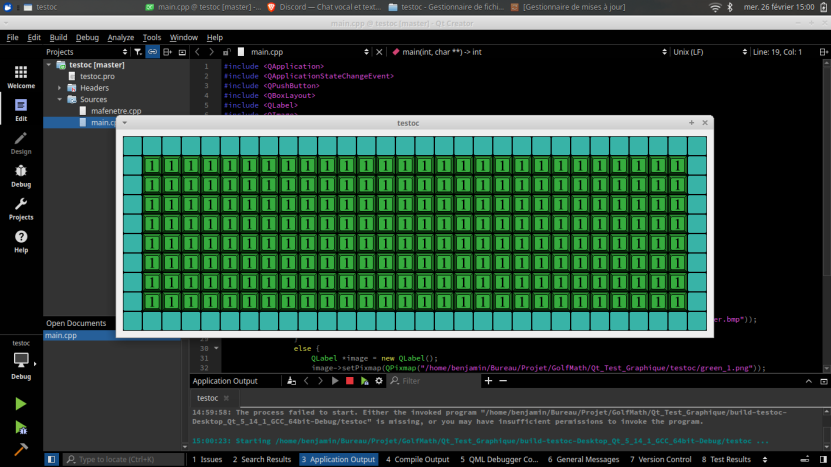
\includegraphics[scale=0.3]{Images/terrain.jpg}
\caption{Premier test de terrain}
\end{figure}
~\\~\\
Le résultat étant trop sombre, on a refait les cases avec un rendu plus clair et plus lisible.\\~\\~\\
\begin{figure}[!h]
\centering

\includegraphics[scale=2]{Images/green.jpg}

\includegraphics[scale=2]{Images/water.jpg}

\includegraphics[scale=2]{Images/hole.jpg}

\includegraphics[scale=2]{Images/start.jpg}
\caption{Rendu deuxième version}
~\\
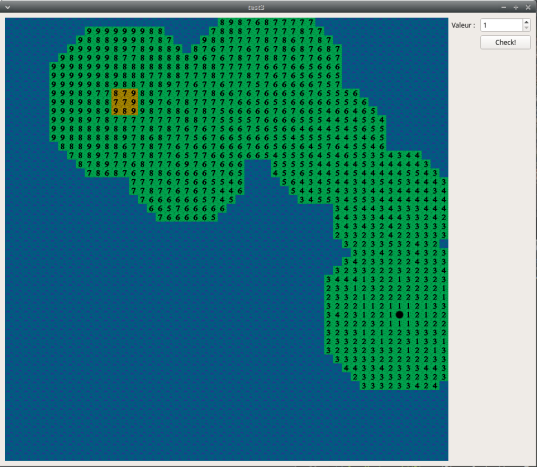
\includegraphics[scale=0.5]{Images/terrain2.jpg}
\caption{Rendu final}
\end{figure}
\newpage
\begin{figure}
\centering

\includegraphics[scale=0.05]{Images/Qt_logo.png}
\end{figure}
\subsection{Qt}
~\\~\\
\textbf{\large La création d'une interface}
\\~\\
Pour pouvoir créer une interface graphique, on utilise la librairie et les objets de Qt, tel que QApplication qui permet de gérer l'interface graphique de l'utilisateur (ou GUI en anglais), ainsi que de contrôler le flux d'entrée et de sortie et les paramètre principaux de notre interface.\\
Voilà à quoi ressemble le code principal pour créer une fenêtre :\\
\begin{verbatim}
#include <QApplication>
#include "toutenun.h"
#include "mainwindow.h"

int main(int argc, char *argv[])
{
    QApplication app(argc, argv);

    MainWindow fen;
    fen.show();

    return app.exec();
}
\end{verbatim}
~\\
\begin{verbatim}
QApplication app(argc, argv);
return app.exec();
\end{verbatim}
~\\
C'est cela qui va créer une première fenêtre.\\
Ensuite les autres objets que nous appellerons, hériteront de la classe QObject, une autre classe importante de Qt qui permet l'affichage de widget.\\
\begin{verbatim}
MainWindow fen;
fen.show();
\end{verbatim}
Cela appelle notre classe MainWindow qui est la fenêtre d'accueil de notre jeu.\\~\\
\begin{figure}[!h]
\centering 
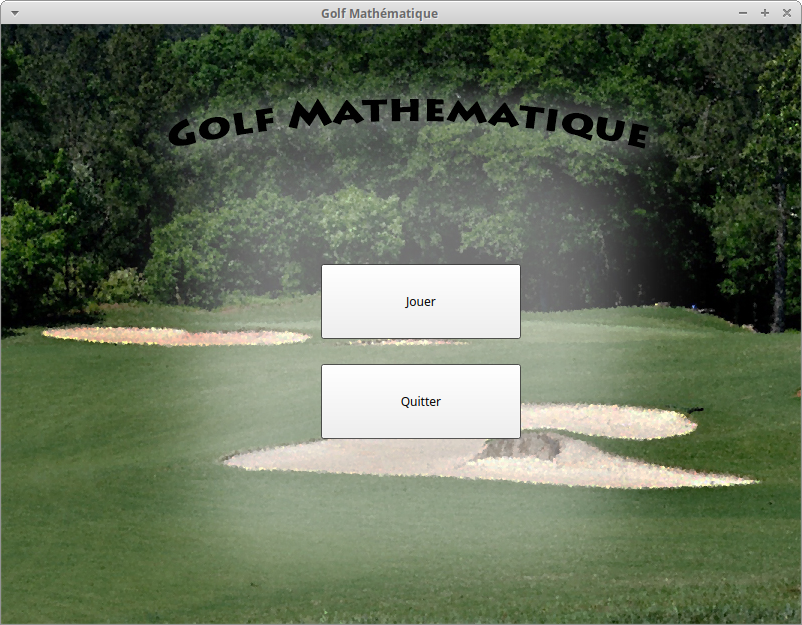
\includegraphics[scale=0.3]{Images/accueil.png}
\caption{Accueil}
\end{figure}
~\\
La classe de cette fenêtre est :
\begin{verbatim}
#include "mainwindow.h"

MainWindow::MainWindow(QWidget *parent) : QMainWindow(parent)
{
    setWindowIcon(QIcon("./image/ballegolf.png"));
    setWindowTitle("Golf Mathématique");
    setFixedSize(800, 600);
    QPalette fond;
    fond.setBrush(backgroundRole(), QBrush(QPixmap("./image/v2/background.jpg")));
    setPalette(fond);

    jouer = new QPushButton("Jouer", this);
    quitter = new QPushButton("Quitter", this);
    jouer->setFixedSize(200, 75);
    quitter->setFixedSize(200, 75);
    jouer->move(320, 240);
    quitter->move(320, 340);

    connect(jouer, SIGNAL(clicked()), this, SLOT(lancer()));
    connect(jouer, SIGNAL(clicked()), this, SLOT(close()));
    connect(quitter, SIGNAL(clicked()), qApp, SLOT(quit()));
}


void MainWindow::lancer()
{
    Niveaux *niv = new Niveaux;
    niv->show();
}
\end{verbatim}
~\\
Ici nous pouvons voir plusieurs nouvel chose. 
\begin{verbatim}
	setWindowIcon(QIcon("./image/ballegolf.png"));
    setWindowTitle("Golf Mathématique");
    setFixedSize(800, 600);
    QPalette fond;
    fond.setBrush(backgroundRole(), QBrush(QPixmap("./image/v2/background.jpg")));
    setPalette(fond);
\end{verbatim}
Toute cette partie s'occupe de l'apparence de la fenêtre, son nom et son icône.
\begin{verbatim}
    jouer = new QPushButton("Jouer", this);
    quitter = new QPushButton("Quitter", this);
    jouer->setFixedSize(200, 75);
    quitter->setFixedSize(200, 75);
    jouer->move(320, 240);
    quitter->move(320, 340);
\end{verbatim}
Celle ci s'occupe des widgets comme les boutons.
\begin{verbatim}
    connect(jouer, SIGNAL(clicked()), this, SLOT(lancer()));
    connect(jouer, SIGNAL(clicked()), this, SLOT(close()));
    connect(quitter, SIGNAL(clicked()), qApp, SLOT(quit()));
\end{verbatim}
Ensuite, on attribut un effet à nos boutons.
\begin{verbatim}
void MainWindow::lancer()
{
    Niveaux *niv = new Niveaux;
    niv->show();
}
\end{verbatim}
Et enfin, cette méthode appelle notre nouvel fenêtre qui gère nos différents niveaux.\\
\begin{figure}
\centering
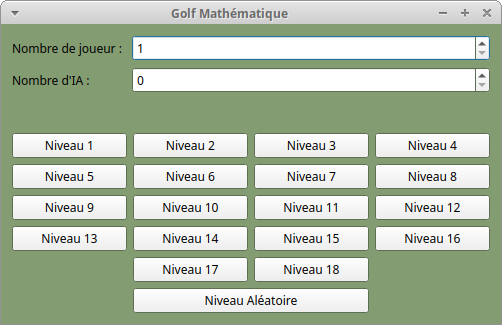
\includegraphics[scale=0.5]{Images/niveaux.png}
\caption{Page des niveaux}
\end{figure}
Les niveaux lance alors différentes seeds (référence des niveaux). Prenons comme exemple le niveau 1 :
\begin{figure}
\centering
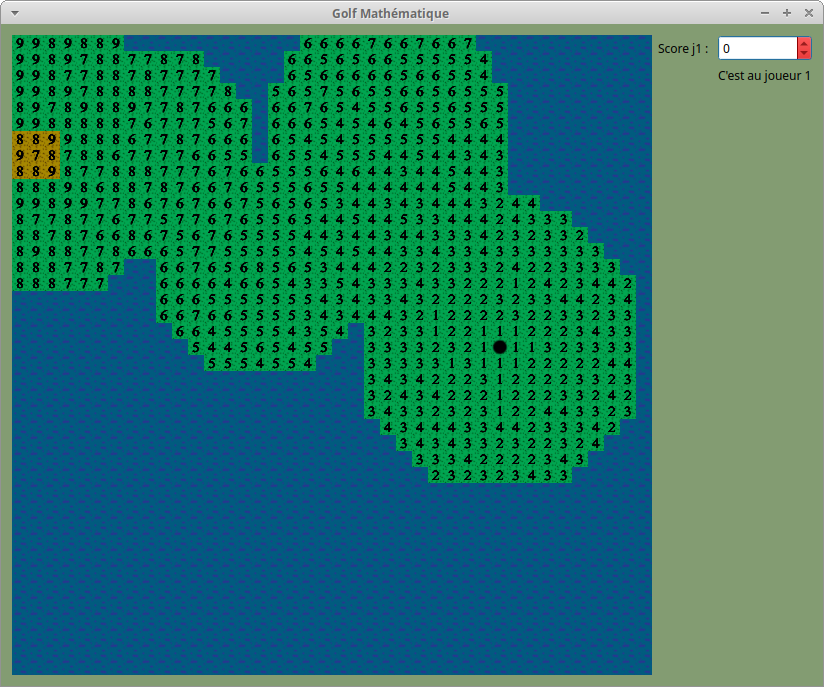
\includegraphics[scale=0.3]{Images/niveau1.png}
\caption{Niveau 1}
\end{figure}
\newpage
\subsection{Intelligence Artificielle - IA}
\subsubsection{Une IA pas très futée}
La première idée pour faire l'ia était de faire une ia des plus basiques qui avance tout droit vers le trou sans réfléchir. l'idée était de, a chaque coup calculer simplement le coup qui rapprochait le plus du trou avec une boucle for très simple.\\
Un problème en est ressorti, c'est très peu efficace. J'ai donc décidé de reprendre du début.\\
\subsubsection{Une IA un peu plus complexe}
Et donc après avoir cherché des algorithme de pathfinding sur internet un algo en particulier ressortais assez souvent : A* (ou A star)\\
C'est un algorithme de pathfinding très connu qui ressemble a ceci :
\begin{verbatim}
Fonction cheminPlusCourt(g:Graphe, objectif:Nœud, depart:Nœud)
       closedList = File()
       openList = FilePrioritaire(comparateur=compare2Noeuds)
       openList.ajouter(depart)
       tant que openList n'est pas vide
           u = openList.depiler()
           si u.x == objectif.x et u.y == objectif.y
               reconstituerChemin(u)
               terminer le programme
           pour chaque voisin v de u dans g
               si non(v existe dans closedList ou si v existe dans openList avec un cout inférieur)
                    v.cout = u.cout +1 
                    v.heuristique = v.cout + distance([v.x, v.y], [objectif.x, objectif.y])
                    openList.ajouter(v)
           closedList.ajouter(u)
       terminer le programme (avec erreur)
\end{verbatim}
J'ai ensuite du évidemment adapter l'algo a notre projet, pour se faire j'ai d'abord du créer une classe qui a une node associe un cout (le nombre de coups jusqu'ici), une heuristique (la distance "a vol d'oiseau" jusqu'à l'arrivée) et un père, pour a la fois pouvoir recréer le chemin après le pathfinding mais aussi tout simplement pour le bon fonctionnement de l'algo. \\
Et après moult complications cette IA était enfin terminée et fonctionelle. A savoir que, bien que l'IA trouve le meilleur chemin a chaque fois, elle n'est pas invincible, il n'est pas compliqué de faire égalité ou même de la battre car j'ai fais en sorte qu'elle ne choisisse pas son point de départ de manière optimale.
\newpage
\subsection{Génération du Terrain}
\subsubsection{Génération Automatique}
Pour générer un terrain de manière automatique on doit place des règles:
\begin{itemize}
\item Le Terrain doit être connexe ou au moins cheminable.
\item La génération des portée doit être presque linéal.

\end{itemize}
Après avoir testé différents idées, nous avons trouvé une solution très convenable pour construire un terrain. Pour générait notre terrain on va produire un chemin est sur celui la on va faire apparente la surface.\\
Cette algorithme est divise en deux passage sur une grille:\\~\\
\textbf{\Large{Premier Passage}}\\
On produit un premier point de manière aléatoire ($P_{x,y}$), et à partir de ce point on génère n-1 autres points ($P_{x,y}$,...,$Pn_{x_n,y_n}$).
\begin{center}
	$k\leq$ n et $k>0, P_{k} = P_{k-1} + \lambda(a, b)$
\end{center}
Telle que le vecteur (a, b)$\in$V, avec V l'ensemble des 7 différents directions valides représente avec des vecteurs.
\begin{center}
	V=\{(-1,-1),(-1,0),...,(1,1)\}\\
	Et $\lambda = B_i$ avec B = \{n-1,n-1,n-2,n-3,...,4,3,2,2\}.
\end{center}
Avec cette algorithme ont trouverait que:\\~\\
X:"l'ensemble des terrains générés" \\
Y:"l'ensemble des chemins possibles"\\
\(\forall x \in X, \exists y \in Y\) telle que "y" est un chemin valide.\\~\\
Avec cette phrase on pouvais générer le terrain sans avoir a penser aux possibles contraintes comme la connexité.
\newpage
\textbf{\Large{Pseudo Code}}\\~\\
\begin{algorithm}[H]
	\caption{GénérationChemin(d lo: entier, d la: entier,d n: entier): Tableau d'entier}
	\SetKwInOut{Parameter}{variables}
	\SetKwInOut{Debut}{début algorithme}
	\SetKwData{I}{i}\SetKwData{LO}{lo}\SetKwData{LA}{la}
	\SetKwData{DIR}{dir}\SetKwData{Va}{v.x}\SetKwData{Vb}{v.y}
	\SetKwData{V}{v}
	\SetKwArray{TAB}{Tab}\SetKwData{N}{n}
	\SetKwFunction{Random}{random}\SetKwFunction{GDIR}{getdirection}
	\SetKwFunction{NPOS}{nouvelPosition}	
	\Parameter{Tab: tableau d'entier bidimensionnel de taille n*m.\\
	i: entier.\\
	v: structure vecteur contenant une paire d'entier\\ "x" et "y".}
	\Debut\\
	\BlankLine
	\I $\leftarrow 1$\;
	\tcp{on définit v le premier point du chemin.}
	\Va $\leftarrow$ \Random{}$\%$($\frac{lo}{2}$)\;
	\Vb $\leftarrow$ \Random{}$\%$($\frac{la}{2}$)\;
	\TAB{\Va}$[$\Vb$]$ $\leftarrow$ 1\;
	\While{\I $<$ \N}
	{
		\DIR $\leftarrow$ \GDIR{}\;\tcp{renvoi un nombre entre {0-7} aléatoirement, qui représente les 8 diffèrent directions}
		\V $\leftarrow$ \NPOS{\V ,\DIR}\;\tcp{renvoi un vecteur qui représente la nouvel position $v_{n+1}$ par rapport a la direction et la position $v_{n}$;}
		\If{\V est valide $\&\&$ \TAB{\Va}$[$\Vb$]$ $==$ 0}
		{
			\TAB{\Va}$[$\Vb$]$ $\leftarrow 1$\;
		}
	}
	\Return \TAB\;
\end{algorithm}
~\\~\\
\newpage
Cette algorithme va nous rendre un tableau d'entier, le quelle on peut représente avec un graph:\\
GénérationTerrain(n,m,5);\\
\begin{figure}[h]
\centering
\begin{tikzpicture}
%nodes
\node [draw, rectangle,label = "Terrain"
		,minimum size = 3cm] (map) 
{
\begin{tikzpicture}
	\foreach \point [count=\i] in {(-5,4),(-4,5.2),(-3,4),(-2,2.5),(-3,1)}
	{
	\fill \point circle (2pt);
	\draw[black, thick] \point circle (1cm);
	\draw[red] \point+(0,0.5) node {$\i$};
	}
\end{tikzpicture}
};
\end{tikzpicture}~\\
\caption{les cercles représente la zone ou le Terrain va ce générait.Anexe 0.}
\end{figure}
\newpage
\definecolor{color1}{RGB}{166,65,180}
\definecolor{color2}{RGB}{55,91,3}
\textbf{\Large{Deuxième Passage}}\\
Déjà générait le chemin, on va passer case par case de notre grille et on va teste si la distance entre la case est un point du chemin est inférieur a un certain nombre.
\begin{center}
On pose (x, y) une case.\\
T l'ensemble des points du chemin.\\
$\lambda$ le rayon.\\
Si distance((x, y), $T_i$) $< \lambda$ alors la case est valide.
\end{center}
si une case est valide ça veut dire que cette case est partie de la surface de notre terrain, donc on doit lui donne une porté, cette porté est définit par la formule suivant:
\begin{center}
	porté = {\color{color1}$(2 + (\frac{dist*8}{sranyon}\%8))$} + 
	{\color{color2}$(((rand()\%5)-2)\%2)$}
\end{center}
Cette formule est divisé on 2 partie, représente par les couleur:
\begin{center}
	1.~~~~~ $(2 + (\frac{dist*8}{sranyon}\%8))$
\end{center}
\textbf{dist} est la distance entre le dernier point du chemin et la case actuel.\\
\textbf{srayon} est la distance entre le dernier point du chemin et le point valide le plus éloigner du dernier point du chemin.\\
A l'aide de GeoGebra on peut représenter cette formule de manière plus graphic.\\
\begin{figure}[!h]
\centering
 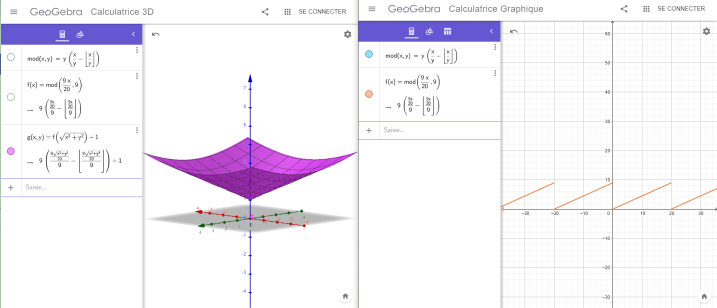
\includegraphics[scale=0.5]{Images/Geogebraimg1.png}\\
 \caption{srayon $=$ 20, 9 au lieu 8 et 1 au lieu 2. La portée d'un point est équivalent a l'axe z.}
\end{figure} 
\begin{center}
	2.~~~~~ $(((rand()\%5)-2)\%2)$\\
\end{center}
rand() un nombre aléatoire entre 0 et RAND{\_}MAX(un nombre très grand qui dépens du langage);
\begin{center}
 $rand()\%5 \leftarrow$ est un nombre entre 0 et 4\\
 $((rand()\%5)-2) \in\{-2,-1,0,1,2\}$\\~\\
 3 nombre pair(60$\%$) et 2 nombre impair(40$\%$).\\~\\
 $(((rand()\%5)-2)\%2) \in\{-1,0,1\}$,\\~\\
\end{center}
ça veut dire qui est plus probable d'avoir 0 que 1 ou -1 donc 60$\%$ de probabilité de ne pas modifier et 40$\%$ pour modifier.

\begin{center}
\textbf{\Large{Pseudo Code}}
\end{center}
\begin{algorithm}[H]
	\caption{GénérationTerrain(d Tab: tableau d'entier,d Ch:tableau de vecteur(les points du chemin),d lo:entier,d la:entier): Tableau d'entier}
	\SetKwInOut{Parameter}{variables}
	\SetKwInOut{Debut}{début algorithme}
	\SetKwData{X}{x}\SetKwData{LO}{lo}\SetKwData{LA}{la}
	\SetKwData{Y}{y}\SetKwArray{CH}{Ch}\SetKwData{EXT}{ext}
	\SetKwArray{TAB}{Tab}
	\SetKwFunction{Random}{random}\SetKwFunction{INRAD}{dansRayon}
	\SetKwFunction{FEXTREM}{extrem}	\SetKwFunction{PORTEE}{calcPortee}	
	\Parameter{}
	\Debut\\
	\BlankLine
	\EXT $\leftarrow$ \FEXTREM{\TAB}\;
	\tcp{renvoi le point le plus éloigner du dernier point du chemin(Ch[n-1]).}
	\For{$\X \leftarrow 0$ \KwTo \LO}
	{
		\For{$\Y \leftarrow 0$ \KwTo \LA}
		{
		\BlankLine
			\If{\INRAD{\TAB{\X}$[$\Y$]$,\CH} et \TAB{\X}$[$\Y$]$ $\notin$ \CH}
			{
				\tcp{dansRayon renvoi vrai ou faux dépendant si un point (x, y) est dans le rayon d'un point du chemin.}
				\TAB{\X}$[$\Y$]$ $\leftarrow$ \PORTEE{\EXT ,\CH{n-1},\TAB{\X}$[$\Y$]$}\;
				\tcp{calcPortee renvoi la porte d'un point utilisant la formule vue avant.}
			}
		}
	}
	\Return \TAB\;
\end{algorithm}
\begin{center}
\begin{tikzpicture}
%nodes
\node [draw, rectangle,label = "Terrain"
		,minimum size = 3cm] (map) 
{
\begin{tikzpicture}
	\foreach \point [count=\i] in {(-5,4),(-4,5.2),(-3,4),(-2,2.5),(-3,1)}
	{
	\draw[black, fill] \point circle (1.5cm);
	}
\end{tikzpicture}
};
\end{tikzpicture}~\\
figure 0: les zones noire représenter la surface jouable.Anexe 0.
\end{center}
\newpage
\section{Bibliographie}
\section{Annexes}
\end{document}
